\documentclass[12pt  , a4, titlepage]{article}
\usepackage[T1]{fontenc}
\usepackage[utf8]{inputenc}
\usepackage[english,italian]{babel}
\usepackage{fancyhdr}

\usepackage[cc]{titlepic}
\usepackage{graphicx}
\usepackage{amsmath}
\usepackage{amsfonts}
\usepackage{multirow}
\usepackage{subfig}
\usepackage{booktabs}
\usepackage[makeroom]{cancel}

\usepackage[autostyle,italian=guillemets]{csquotes}

\usepackage{lipsum}

\usepackage{quoting}
\quotingsetup{font=small}


\usepackage{hyperref}
\hypersetup{colorlinks,
	linkcolor = black,
	urlcolor  = black,
	citecolor = black,
	anchorcolor = black,
	linktocpage}

\usepackage[scaled=0.92]{helvet}
\usepackage[sf]{titlesec}
\usepackage{rotating}

\newcommand{\E}{\`E }

\newcommand{\norm}[1]{\left\lVert#1\right\rVert}

\addto\captionsitalian{\renewcommand{\figurename}{Fig.}}
\addto\captionsitalian{\renewcommand{\tablename}{Tab.}}

\usepackage[nottoc,notlot,notlof]{tocbibind}
\addto\captionsitalian{\renewcommand{\listfigurename}{Indice delle figure}}
\addto\captionsitalian{\renewcommand{\listtablename}{Indice delle tabelle}}

\title{MANUALE SEZTORSIONE}
\date{}
\titlepic{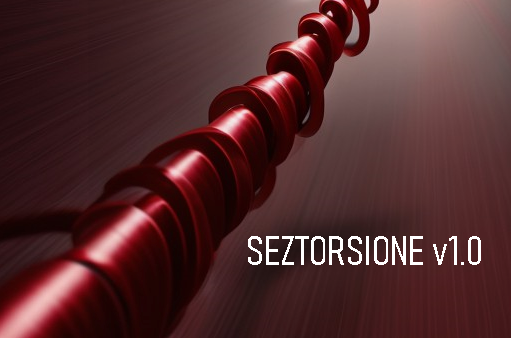
\includegraphics[width=\textwidth]{../SPLASH}}
\begin{document}

	\maketitle

	\section*{INTRODUZIONE}
	Si spiega brevemente come inserire i dati nei file di input.
	
	\section*{SEZIONE.CSV}
	\begin{figure}[h!]
		\centering
		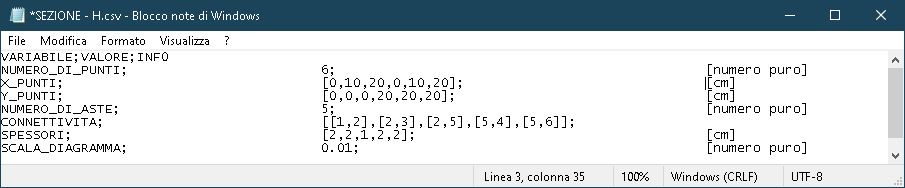
\includegraphics[width=\linewidth]{FIGURE/SEZIONE_TOT}
		\caption{}
		\label{fig:sezionetot}
	\end{figure}
	\subsection*{NUMERO PUNTI}
	Specificare il numero di punti che compongono la sezione. Ad esempio una sezione a doppio T è composta da 6 punti. Una sezione a C è composta da 4 punti (vedi figura sotto).
	
		\begin{figure}[h!]
		\centering
		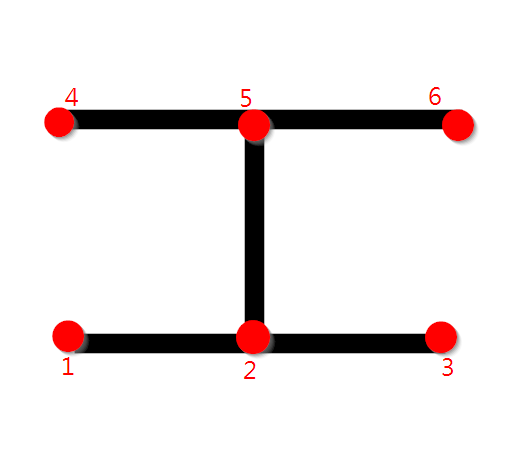
\includegraphics[width=0.5\linewidth]{FIGURE/NUM_NODI}
		\caption{}
		\label{fig:NUM_NODI}
	\end{figure}

\subsection*{X PUNTI}
	Si mette la coordinata X dei punti. L'ordine è:
	\[
	[x_{punto1}, x_{punto2}, \dots , x_{punto i} , \dots, x_{puntoN}]
	\]
	\subsection*{Y PUNTI}
	Si mette la coordinata Y dei punti. L'ordine è:
	\[
	[y_{punto1}, y_{punto2}, \dots , y_{punto i} , \dots, y_{puntoN}]
	\]
	\subsection*{NUMERO DI ASTE}
	\E il numero di segmenti rettilinei che compongono la sezione. Ad esempio una sezione a doppio T è composta da 5 aste, una sezione a C è composta da 3 aste (vedi figura sotto)
.
		\begin{figure}[h!]
	\centering
	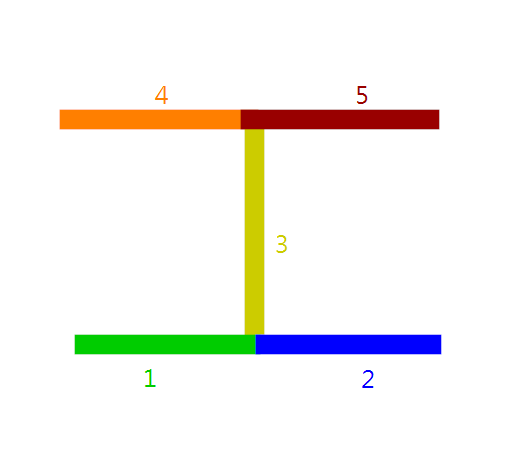
\includegraphics[width=0.5\linewidth]{FIGURE/NUM_ASTE}
	\caption{}
	\label{fig:NUM_ASTE}
\end{figure}

\subsection*{CONNETTIVITA}
	Questo è il punto fondamentale. Se si sbaglia la connettività della sezione il programma non funziona.
	
	All'interno delle parantesi quadre si deve scrivere una lista di coppie di numeri. Questi numeri sono i nomi dei nodi che vengono collegati dalle aste. Ad esempio l'asta 3 della figura precedente va dal nodo 2 al nodo 5, dunque si  scriverà:
	\[
	[[I1,J1],[I2,J2], [2,5],\dots]
	\]
	\E FONDAMENTALE CHE CIASCUN NODO RISULTI ESSRE NODO DI ARRIVO SOLAMENTE PER UN ASTA, nella figura seguente viene illustrato il significato di questa frase.
	
			\begin{figure}[h!]
		\centering
		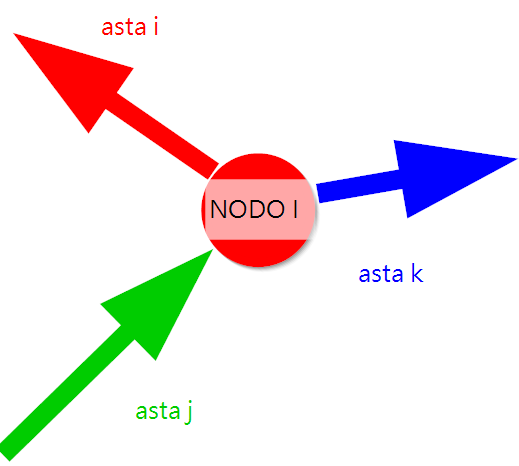
\includegraphics[width=0.5\linewidth]{FIGURE/CONNETTIVITA_GIUSTA}
		\caption{Definizione corretta della connettività.}
		\label{fig:CONNETTIVITA_GIUSTA}
	\end{figure}
\begin{figure}[h!]
	\centering
	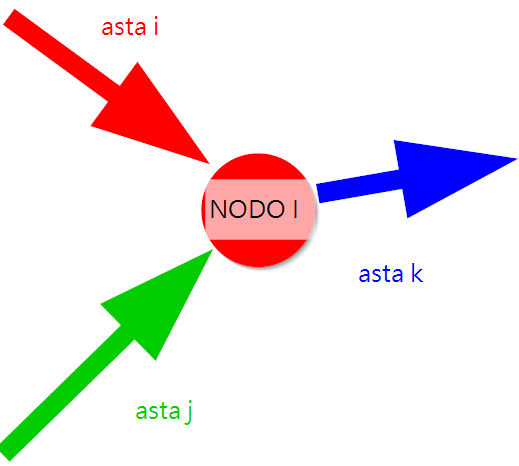
\includegraphics[width=0.5\linewidth]{FIGURE/CONNETTIVITA_SBAGLIATA}
	\caption{Definizione sbagliata della connettività.}
	\label{fig:CONNETTIVITA_SBAGLIATA}
\end{figure}

	Se in un unico nodo convergono due o più aste il software non funziona e restituisce un errore.

\subsection*{SPESSORI}
Sono gli spessori delle aste, quindi è una lista di numeri. La lista è composta da un numero di valori pari al numero di aste. 
\subsection*{SCALA DIAGRAMMA}
Serve a riscalare il diagramma della funzione di ingobbamento che potrebbe essere troppo grande o troppo piccolo. Andando per tentativi si può trovare la visualizzazione piu corretta.
	\newpage+
	\section*{SCHEMA STATICO.CSV}
	\begin{figure}[h!]
		\centering
		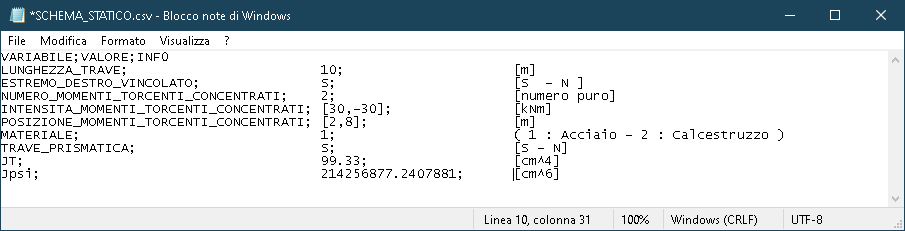
\includegraphics[width=\linewidth]{FIGURE/SCHEMA STATICO_TOT}
		\caption{}
		\label{fig:SCHEMA STATICO_TOT}
	\end{figure}
	\subsection*{LUNGHEZZA TRAVE}
	Si specifica la lunghezza della trave in metri.
	\subsection*{ESTREMO DESTRO VINCOLATO}
	Se l'estremo destro è vincolato la trave avrà vincolo sia a sinistra che a destra come nella seguente figura.
	
		\begin{figure}[h!]
		\centering
		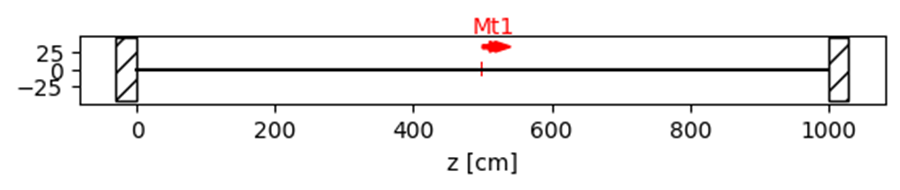
\includegraphics[width=\linewidth]{FIGURE/DOPPIO INCASTRO}
		\caption{}
		\label{fig:SCHEMA DOPPIO INCASTRO}
	\end{figure}

	Altrimenti la trave è incastrata solo a sinistra.
	
		\begin{figure}[h!]
		\centering
		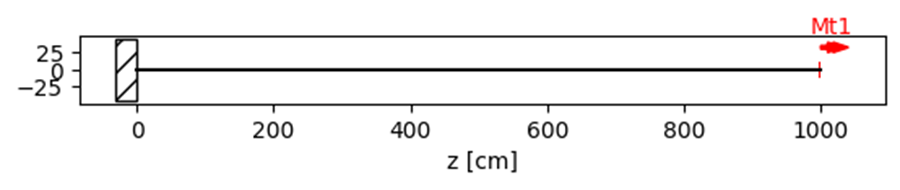
\includegraphics[width=\linewidth]{FIGURE/SINGOLO INCASTRO}
		\caption{}
		\label{fig:SCHEMA SINGOLO INCASTRO}
	\end{figure}

	\subsection*{NUMERO MOMENTI TORCENTI CONCENTRATI}
	Il numero di momenti torcenti lungo la trave.
	\subsection*{INTENSITA MOMENTI TORCENTI CONCENTRATI}
	L'intensità dei moemnti torcenti lungo la trave in kNm.
	\subsection*{POSIZIONE MOMENTI TORCENTI CONCENTRATI}
		La posizione è sempre data a partire dal nodo sinistro. Lo schema è quello della seguente figura.
		
			
		\begin{figure}[h!]
			\centering
			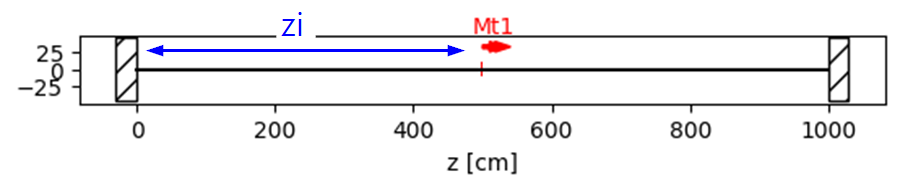
\includegraphics[width=\linewidth]{FIGURE/POSIZIONE CARICHI}
			\caption{}
			\label{fig:POSIZIONE CARICHI}
		\end{figure}
	
	\subsection*{MATERIALE}
	\E acciaio oppure calcestruzzo. Le proprietà del calcetruzzo non vengono calcolate in base alla classe ma sono fissate pari a E=30000MPa eG=15000MPa.
	
	\subsection*{TRAVE PRISMATICA}
	Se la trave è prismatica allo è a sezione costante e basta indicare solamente un valore di Jt e uno di J$\psi$. Altrimenti bisognerà fare una lisa di valori del tipo [Jt del tratto 1, Jt del tratto 2 ,Jt del tratto 3, ...].
	
	\subsection*{JT}
	Jt relativo alla torsione primaria. Di fatto è:
	\[
	J_t=\sum_{i=1}^{Naste}\frac{s_i^3*L_i}{3}
	\]
	\subsection*{J$\psi$}
	\E il modulo di inerzia settoriale. La formula generale è:
	\[
	J_{\psi} = \int_A \psi^2 dA
	\]
	Di fatto è calcolato con la teoria delle aree settoriali.
	
\end{document}